\documentclass[runningheads]{llncs}

\usepackage{graphicx}
\usepackage{todonotes}
\usepackage{listingsutf8}
\usepackage[hidelinks]{hyperref}
\usepackage{cleveref}
\usepackage{footmisc}
\usepackage{bookmark}

\renewcommand\UrlFont{\color{blue}\rmfamily}

\begin{document}

\title{L4DR: A 2nd-gen, national GeoLD system}
\titlerunning{Loc-I for Disaster Recovery}

\author{
    Nicholas J. Car\inst{1}\orcidID{0000-0002-8742-7730} \and \\
    Irina Bastrakova\inst{2}\orcidID{0000-0002-4643-7289}
}

\authorrunning{Car N.J. et al.}

\institute{
    {
    SURROUND Australia Pty Ltd., Australia \&\\
    Australian National University, Australia\\
    \email{nicholas.car@surroundaustralia.com}
    %\url{https://surroundaustralia.com}
    }
    \and
    {
        Geoscience Australia\\
        \email{irina.bastrakova@ga.gov.au}
    }
}

\maketitle

\begin{abstract}
Increasingly, multiple sources of data are available for disaster recovery planning and emergency service scheduling. Data sharing systems may
have to simultaneously cover multiple diverse use cases (e.g. social, environmental and economic) and be transparent, verifiable and trusted. 
The 2020 Australian bushfire crisis and the global COVID-19 pandemic are examples of complex crisis events where lots of data sources are available.\\

In 2018 – 2020, Australia built several \textit{Linked Data} ``spines'' - themed collections of interoperable reference data that simplify data 
integreation in particular domains. 
The spatial data spine, Loc-I (Location Index), initially consisted of three nationally-significant spatial datasets, such as the \textit{Australian Statistical Geography Standard}. 
Loc-I delivers Linked Data forms of its datasets and provided infrastructure for their use as a single system.\\

Here we describe \textit{Loc-I for Disaster Recovery}, a scenario deployment extension for Loc-I.
We discuss original Loc-I design, this project's differences and its different key requirements, isuch as to integrate Linked Data with traditional
spatial data systems, and how this system is pushing spatial and \textit{Semantic Web} standards development such as DGGS and GeoSPARQL.

\keywords{Location Index \and Loc-I \and GeoSPARQL \and DGGS \and Spatial Data on the Web \and Australia \and national data infrastructure}
\end{abstract}


\section{Introduction}\label{sec:introduction}
\subsection{Motivation}
Australia suffers large floods and bushfires, so the Australian government is committing substantial resources over 
multiple years to new cross-agency data sharing initiatives\footnote{``Australia commits to climate resilience'', 
\url{https://minister.awe.gov.au/ley/media-releases/australia-commits-climate-resilience}}, 
which will ``connect and leverage the Commonwealth’s extensive climate and natural disaster risk information to further prepare for and build resilience to natural disasters''.

\subsection{Demonstrator Projects}
Several demonstrator projects for an anticipated new data sharing regime were conducted in early 2021. 
Traditional methods of data aggregation are being tested, such as data pooling in shared facilities,
standardising web services and cross-cataloging datasets, and also forward-looking methods. In particular,
\textit{Semantic Web} (SW) and \textit{Linked Data} (LD) technologies\footnote{By ``Linked Data'', as opposed to ``linked data'' or ``data linkage'' etc.,
we mean systems and data that implement a number of \textit{Semantic Web} technologies (RDF, OWL, SKOS, SPARQL, etc.), primarily 
defined by a series of \href{https://www.w3.org/standards/semanticweb/data}{World Wide Web Consortium} (W3C) standards. The W3C's defintion of 
\textit{Semantic Web} is that it is a ``Web of Data'', an evolved Internet able to be queried by machineswhich can draw inferences from it.}
are being used to integrate different, but relatively similar, datasets that are published in a distributed manner and
spatial data methods using a \textit{Discrete Global Grid System} (DGGS) are being used to integrate spatial data from multiple sources. In 2019-2020, Geoscience Australia tested DGGS data integration
for information relevant to bushfires which includes burned/burning areas, vegetation cover and demographics.

This paper describes the SW/LD and DGGS approaches to publish distributed and harmonised data being implemented by a Geoscience Australia (GA) project that we will 
refere to as \textit{this project}. The project extends the approach taken by the Location Index project described in the next section.

\section{Loc-I: The Location Index}\label{sec:loci}

\begin{figure}[htb]
    \centering
    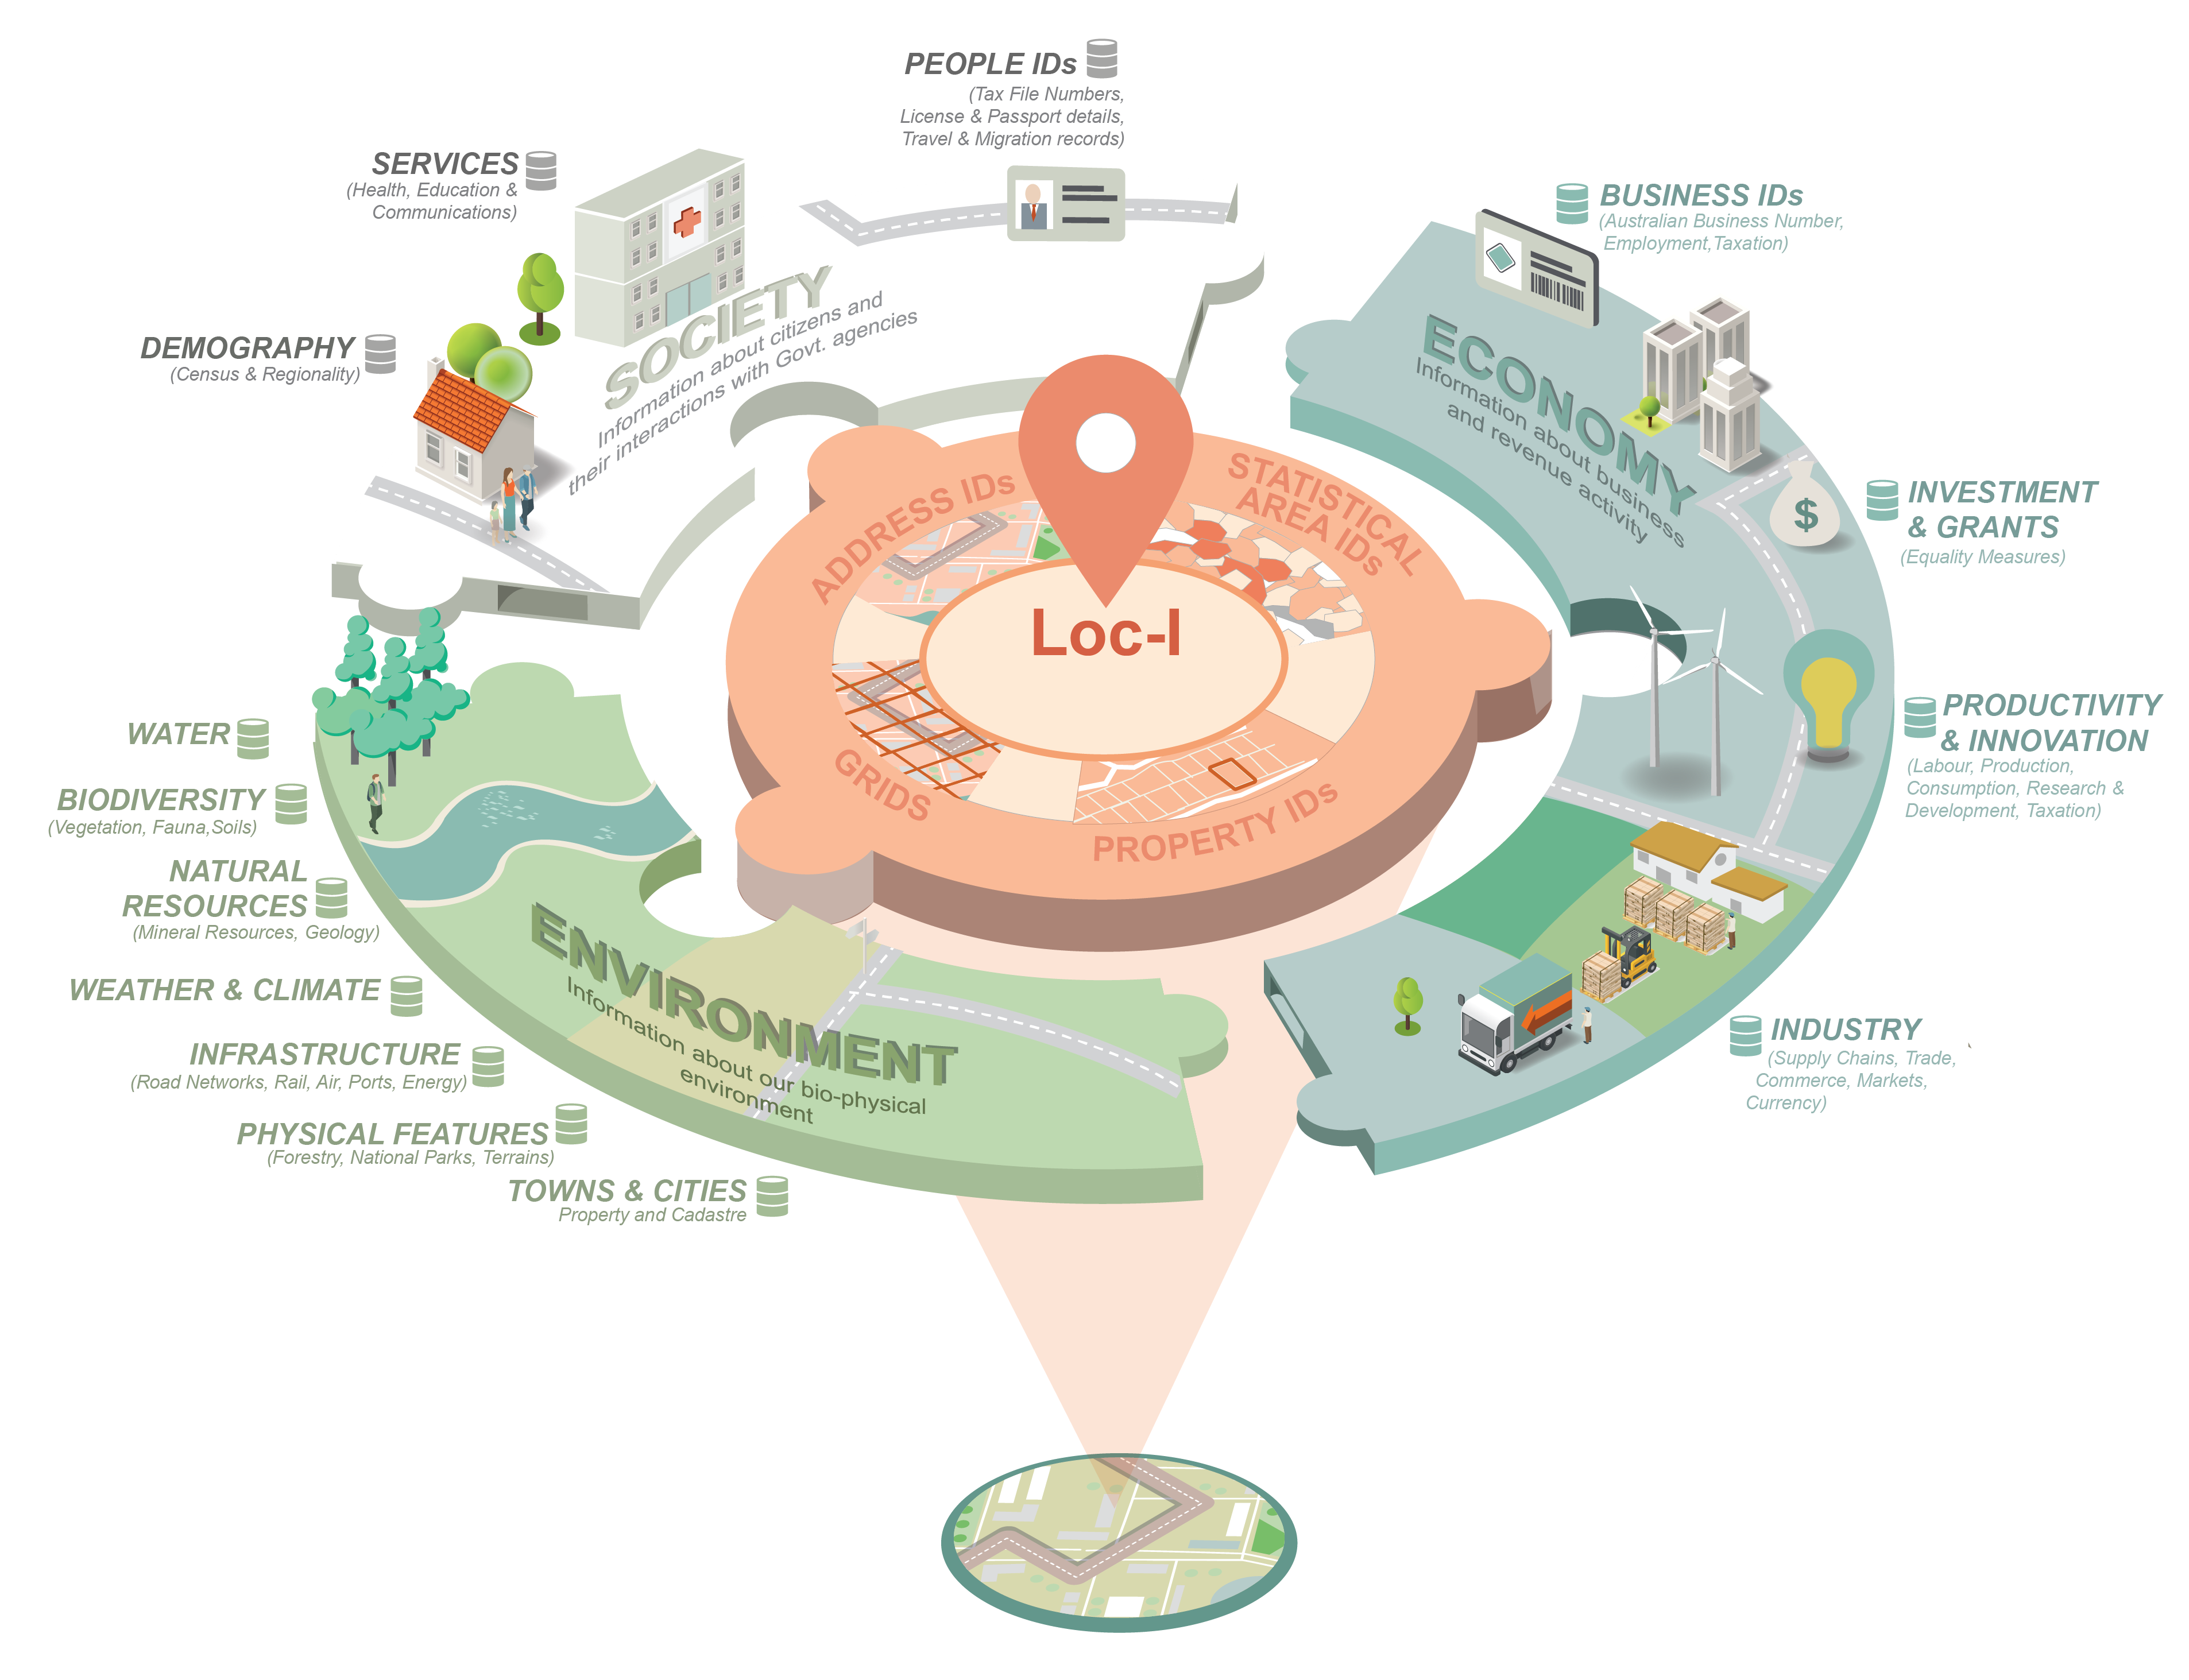
\includegraphics[width=\linewidth]{images/loci-brochure.png}
    \caption{A project brochure image, from \cite{car_location_2019}, of Loc-I with respect to
    Australian government \textit{Environment}, \textit{Society} and \textit{Economy} data}
    \label{fig:loci-brochure}
\end{figure}

In 2018 - 2020, Australian spatial data and research agencies (\href{https://www.csiro.au}{CSIRO} \& \href{https://www.ga.gov.au}{Geoscience Australia} **foring** for the \href{https://www.abs.gov.au}{Australian Bureau of Statistics}) implemented a ``national and authoritative, also federated, index for Australian spatial data using Semantic Web technologies~\cite{car_location_2019}''.

This system, known as the Location Index (Loc-I)~\cite{car_location_2019}, aims to ``better geospatially integrate and analyze data across 
government portfolios and information domains''. The main use case addressed by Loc-I is to greatly reduce the time taken by government 
workers in data analysis using spatial information by providing pre-integrated, authoratitive, spatial datasets that can be used in 
online, open data scenarios, within secure data integration environments and across the two. The project deals with data from multiple domains,
see Figure~\ref{fig:loci-brochure}. Some of the interesting aspects of the Loc-I design include:

\begin{itemize}
    \item[$\ast$] federated publication of datasets via standard Linked Data APIs
    \item[$\ast$] use of VoID \texttt{Linkset}~\footnote{\url{https://www.w3.org/TR/void/}} instances to crosswalk datasets
    \begin{itemize}
        \item[$-$] these are independently-selectable for use meaning that a specific ccrosswalk, of potentially many, may be selected for use
    \end{itemize} 
    \item[$\ast$] use of a \textit{Geometry Data Service}\footnote{The service is online at \url{https://gds.loci.cat/}} for spatial integration
    \begin{itemize}
        \item[$-$] this service extends common use of using GeoSPARQL~\cite{open2012ogc} by storing \texttt{Geometry} instances seperately from the \texttt{Feature} instances they are the geometries for. This allows the geometry data to be managed in a PostGIS database\footnote{\url{https://postgis.net/}}, not a triplestore, as usually used for GeoSPARQL data.
    \end{itemize}
    \item[$\ast$] several different clients for different uses
    \begin{itemize}
        \item[$-$] such as \textit{Excelerator}\footnote{\url{https://loci.cat/excelerator.html}}, used to upload data according to one spatial reference system and download it reapportioned according to another
    \end{itemize}
\end{itemize} 

The Loc-I datasets are from many domains including environmental (the \textit{Australian Hydrological Geospatial Fabric}
\footnote{Original, non-RDF dataset: \url{http://www.bom.gov.au/water/geofabric/}, and the online LD version implemented by Loc-I: \url{http://linked.data.gov.au/dataset/geofabric}}, 
a collection of surface hydrology features), human/census (the \textit{Australian Statistical Geography Standard} spatial areas)
\footnote{Non-RDF dataset: \url{https://geo.abs.gov.au/arcgis/services/ASGS2016/MB/MapServer/WFSServer}, LD version: \url{http://linked.data.gov.au/dataset/asgs2016}}, 
and cartographic/administrative (the \textit{National Composite Gazetteer of Australia})\footnote{LD version: \url{https://linked.data.gov.au/dataset/placenames}}. 

Some details of the Loc-I architectureares shown in Figure~\ref{fig:loci-arch}. It shows the Loc-I Data Cache, which is a multi-graph triplestore, 
obtains its data by ``pulling'' RDF datasets through APIs that both interpret non-RDF data for online delivery and are also able to create static RDF 
versions of the datasets. All Loc-I datasets conform to the Loc-I Ontology\footnote{\url{http://linked.data.gov.au/def/loci}} which imports the GeoSPARQL
\footnote{\url{http://www.opengis.net/doc/IS/geosparql/1.0}} and DCAT\footnote{\url{https://www.w3.org/TR/2014/REC-vocab-dcat-20140116/}} ontologies. 
Alongside the Cache is a traditional spatial DB - PostGIS\footnote{\url{https://postgis.net/}} used to perform fast geometry intersections.

\begin{figure}[htb]
    \centering
    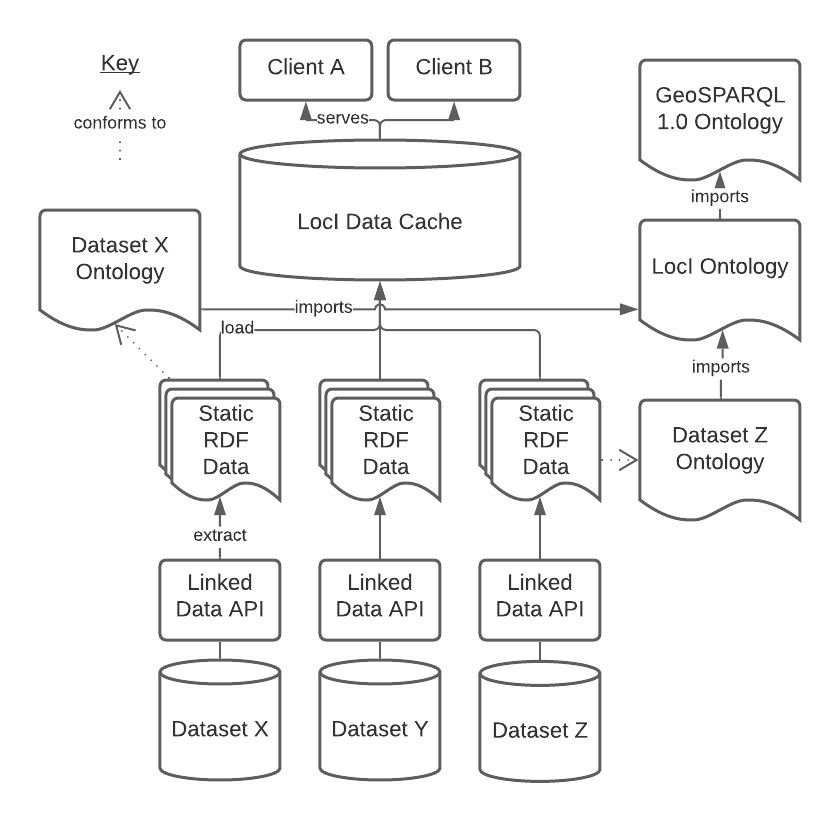
\includegraphics[width=0.8\linewidth]{images/loci-arch.png}
    \caption{An informal architecture diagram of Loc-I's \textit{Linked Data} infrastructure.}
    \label{fig:loci-arch}
\end{figure}

\section{Loc-I for Disaster Recovery}\label{sec:changes}
\subsection{Data Validity}
The project datasets are Loc-I datasets and its Knowledge Graph (KG) is similar to the Loc-I cache, however conformance to Loc-I is not easily
testable: Loc-I provided no data validators. This project implements formal \textit{profiles}, which 
are specifications defining dependencies and validation tooling. This project uses profiles for requirements for data 
publication by API, dataset suitability for the KG and for use and display by clients and they are defined using 
\textit{The Profiles Vocabulary}~\cite{atkinson_profiles_2020} and all listed in the project's LD catalogue\footnote{\label{catalogue} \url{https://w3id.org/l4dr/explorer}}.

\subsection{Use of Discrete Global Grid System (DGGS)}
It was planned for Loc-I to use DGGS geometries\footnote{See the defining \textit{Abstract Specification}~\cite{purss_topic_2017} for indications of potential benefits of 
DGGS and the more recent \textit{OGC Engineering Report}~\cite{gibb_ogc_2021} for current thinking about how to integrate DGGS use within traditional spatial 
infrastructure.} but this has not yet been integrated into the core Loc-I cache. In 2020, Geoscience Australia evaluated DGGS integration of data
relating to bushfires in Australia - vegeration, population and bush fire extent information and from this established some new DGGS integration methods. Also, SURROUND Australia
implemented DGGS data delivery via Linked Data APIs for the OGC,s \textit{Testbed 16} interoperability experiment~\cite{gibb_ogc_2021}.
Using the GA DGGS methods and SURROUND tooling, this project has produced DGGS versions of all \texttt{Feature} instances' 
geometries, has stored them alongside traditional geometries within the KG (a triplestore) and has implemented GeoSPARQL~\cite{open2012ogc} functions
within the triplestore SPARQL extension libraries (Apache Jena's ARC\footnote{\url{https://jena.apache.org/documentation/query/extension.html}}) that work with 
DGGS geometry representations. These functions are used to obviate the need for Loc-I's Geometry Data Store and thus reduce infrastructure complexity.

An important enabling factor in this use of DGGS with GeoSPARQL is the inclusion of DGGS geometry serializations within version 1.1 of GeoSPARQL which was motivated
by Loc-I project requirements. This version is currently under review and is expected to be published around the time of this paper's publication. Working documents 
are available\footnote{See \url{https://opengeospatial.github.io/ogc-geosparql/} for the GeoSPARQL ``Standards Working Groups`` 's working documents}.

\subsection{Observations data use}
Loc-I anticipated observational data - human/industry statistics or natural-world observation data - wuold be used with its spatial data. This project
implements two such datasets: 1. population data taken from the 2016 Australian census; 2. ``exposure'' data per statistical area - this is data about the vulnerability
of physical infrastructure to natural hazards. This project has developed an ``Observations Dataset'' profile (see the project catalogue\footref{catalogue}) that defines the characteristics of a Loc-I-compatible (conformant?)
observations dataset using the profiling mechanisms mentioned above.

\subsection{Knowledge Graph (KG) importing}
This project's KG includes Loc-I datasets as well as new Loc-I-conformant (compatible?) datasets. To avoid duplication, this project intends to import Loc-I content unchanged however, 
currently, the additional requirements this project has (see the listed changes above) mean that Loc-I datasets have to be extended and thus reuse of Loc-I datasets
or the data cache (see Figure~\ref{fig:loci-arch}) is not currently possible. For now, a ``Loc-I 2 KG'' has een created and imported into this project's KG (see 
\ref{fig:l4dr-arch}) but this will be removed when Loc-I implements this project's elements.

\subsection{Data and metadata management}
Operational management of data was out of scope for Loc-I as a technical demonstrator, however, this project
is moving towards a production system that must managed content to assure currency. For this reason, it has implemented a sophsticated application layer on top of its KG, the 
\textit{SURROUND Ontology Platform}\footnote{\url{https://surroundaustralia.com/sop}},  used to track, select for use, update and overall govern datasets. This application
supports provenance absorbtion (for datasets that contain provenance) and generation (for data processing contained within the platform) as well as managed item (dataset, ontology, vocabulary)
status tracking and even the automated calculation of \textit{FAIR Scores}\footnote{Scored for datasets rated against the \textit{FAIR PRinciples}: \url{https://www.go-fair.org/fair-principles/}}.

\subsection{Clients}
Loc-I implemented some generic and specialised clients for its data holdings\footnote{See \url{https://loci.cat/\#datasets-and-applications} for a list}. This project can reuse some, such as 
\textit{IDer Down}\footnote{\url{https://excelerator.loci.cat/iderdown}} - used to download IDs for all \texttt{Feature} type instances - due to the same data structures being used.
However, this project is also charged with demonstrating integration of Linked Data with traditional spatial web data delivery. For this reason, information
flows between a traditional web globe\footnote{TerriaJS (\url{https://terria.io/}) at \url{https://w3id.org/l4dr/globe}}
and a Linked Data browser\footnote{This system allows for the browsing of content within this project's KG as \url{https://w3id.org/l4dr/explorer}, as opposed to the LD dereferencing of individual resources 
which is acomplished by the APIs implemented for each dataset.} with panels of per-\texttt{Feature} information accessible witin the globe supplied by KG queries. Previous spatial web data display
only presents simple type key / value pairs of information per-\texttt{Feature} but this system presents graph data which can be followed. Also, the management requirement, described above, has 
necessitated an adminstrative interface to this project's KG, that Loc-I never had.

\subsection{More standardized Dataset APIs}
Loc-I implemented LD APIs for spatial datasets that followed standard LD protocols and the data model negotiation protocols of \textit{Content Negotiation by Profile} (ConnegP)~\cite{atkinson_profiles_2020}.
Content within these APIs was all discoverable since top-level elements - dataset declarations - linked to their content registers and registers linked to individual \texttt{Features}, 
however no strict or common spatial API structure was used. This project implements APIs as both LD APIs and also as \textit{OGC API: Features}~\cite{clemens_portele_ogc_2019} APIs\footnote{See an example of such an API online at \url{https://w3id.org/l4dr/provinces} or browse the project catalogue, as linked to in previous footnotes}.
This is possible due to ConnegP implementations being able to select data models and formats per API endpoint using general mecahnics (HTTP headers or URI query strings) that can be constrained
to meet OGC API: Features requiements. ConnegP APIs are also used to deliver the observations datasets but these are not conformant with OGC API:Features since they don't contains any geometry 
infromation - they link to spatial datasets' \texttt{Features} for their data's spatial information.

\begin{figure}[htb]
    \centering
    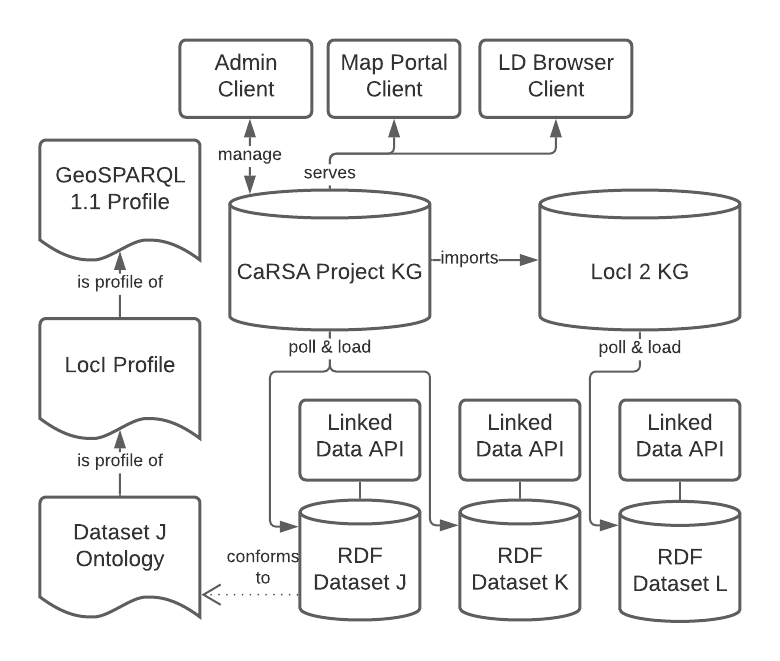
\includegraphics[width=0.8\linewidth]{images/l4dr-arch.png}
    \caption{An informal architecture diagram of the L4DR project's \textit{Linked Data} infrastructure}
    \label{fig:l4dr-arch}
\end{figure}


\section{Conclusions}\label{sec:conclusions}
This project is both re-user and extender of Loc-I systems. Core benefits of spatial Linked Data are preserved - harmonised use of distributed datasets, human- and machine-readable 
web content - and Semantic Web methods - inferencing, ontology modelling however new spatial data indexing is applied (Discrete Global Grid System use), total project data holdings management is
enabled, data validators created and new clients are delivered. The resulting system is a proto-operational system as opposed to a proof-of-concept.


\subsection{Future Work}\label{sec:futurework}
This project will operate in test mode until July 2021. Full production will be highly dependent on 
uninterrupted data supply guarentee currency. To ensure this, inter-agency data supply chain management - stated in the Loc-I project but not completed - 
must be finalised. For data to be delivered by owner agencies as Linked Data, assistance will need to be given to those agncies to be able to make Semantic Web and Linked Data verisions of their data
for delivery via APIs. This will require strong motivation from central government data users to ensure these requirements are met as implementation is a socio-technical challenge, not purely a 
technical one.


%
% ---- Bibliography ----
%
% BibTeX users should specify bibliography style 'splncs04'.
% References will then be sorted and formatted in the correct style.
%
\bibliographystyle{splncs04}
\bibliography{references}
%
% \begin{thebibliography}{8}
% \bibitem{ref_article1}
% Author, F.: Article title. Journal \textbf{2}(5), 99--110 (2016)

% \bibitem{ref_lncs1}
% Author, F., Author, S.: Title of a proceedings paper. In: Editor,
% F., Editor, S. (eds.) CONFERENCE 2016, LNCS, vol. 9999, pp. 1--13.
% Springer, Heidelberg (2016). \doi{10.10007/1234567890}

% \bibitem{ref_book1}
% Author, F., Author, S., Author, T.: Book title. 2nd edn. Publisher,
% Location (1999)

% \bibitem{ref_proc1}
% Author, A.-B.: Contribution title. In: 9th International Proceedings
% on Proceedings, pp. 1--2. Publisher, Location (2010)

% \bibitem{ref_url1}
% LNCS Homepage, \url{http://www.springer.com/lncs}. Last accessed 4
% Oct 2017
% \end{thebibliography}
\end{document}




% Outline
% 
% Section 1
%   History of GeoSPARWL 1.0
% Section 2
%   motivation to update the spec
% Section 3
%   GeoSPARQL 1.1 additions
%       motivation, and expected use, of new spatial functions. In particular, why in GeoSPARQL when aggregations etc. can be performed elsewhere?
%       Spatial Measure
% Section 4
%       new profile presentation
%       new URI regimes etc
% Section 5
%       expected changed use modes
